\chapter{Dataset Profiles and Models}\label{chapter:hdl}
\graphicspath{{part1/chapter1/figures/}}

The value of Open Data is recognized when it is used. To ensure that, publishers need to enable people to find datasets easily. Data portals are specifically designed for this purpose. They make it easy for individuals and organizations to store, publish and discover datasets.

Data models vary across data portals. While exhaustively surveying the range of data models, we did not find any that offers enough granularity to completely describe complex datasets facilitating search, discovery and recommendation. For example, the Datahub uses an extension of the Data Catalog Vocabulary (DCAT)~\cite{Erickson:DCV:14} which prohibits a semantically rich representation of complex datasets like DBpedia\footnote{\url{http://dbpedia.org}} that has multiple endpoints and thousands of dump files with content in several languages~\cite{Brummer::ICSS:14}.

From our survey, we found that a proper integration of Open Data into businesses requires datasets to include the following information:
\begin{itemize}
	\item \emph{Access information}: a dataset is useless if it does not contain accessible data dumps or query-able endpoints;
	\item \emph{License information}: businesses are always concerned with the legal implications of using external content. As a result, datasets should include both machine and human readable license information that indicates permissions, copyrights and attributions;
	\item \emph{Provenance information}: depending on the dataset license, the data might not be legally usable if there are no information describing its authoritative and versioning information. Current models under-specify these aspects limiting the usability of many datasets.
\end{itemize}

%%%%%%%%%%%%%%%%%%%%%%%%%%%%%%%%%%%%%%%%%%%%
%%%  2. Data Portals and Dataset Models  %%%
%%%%%%%%%%%%%%%%%%%%%%%%%%%%%%%%%%%%%%%%%%%%

\section{Data Portals and Dataset Models}
\label{section:datasetModels}
There are many data portals that host a large number of private and public datasets. Each portal present the data based on a model used by the underlying Data Management Software. In this section, we present the results of our landscape survey of the most common data portals and dataset models.

\subsection{DCAT}
The Data Catalog Vocabulary (DCAT) is a W3C recommendation that has been designed to facilitate interoperability between data catalogs published on the Web~\cite{Erickson:DCV:14}. The goal behind DCAT is to increase datasets discoverability enabling applications to easily consume metadata coming from multiple sources. Moreover, the authors foresee that aggregated DCAT metadata can facilitate digital preservation and enable decentralized publishing and federated search.

DCAT is an RDF vocabulary defining three main classes: \texttt{dcat:Catalog}, \texttt{dcat:Dataset} and \texttt{dcat:Distribution}. We are interested in both the \texttt{dcat:Dataset} class which is a collection of data that can be available for download in one or more formats and the \texttt{dcat:Distribution} class which describes the method with which one can access a dataset (e.g. an RSS feed, a REST API or a SPARQL endpoint).

\subsection{DCAT-AP}
The DCAT application profile for data portals in Europe (DCAT-AP)\footnote{\url{https://joinup.ec.europa.eu/asset/dcat\_application\_profile/description}} is a specialization of DCAT to describe public section datasets in Europe. It defines a minimal set of properties that should be included in a dataset profile by specifying mandatory and optional properties. The main goal behind it is to enable cross-portal search and enhance discoverability. DCAT-AP has been promoted by the Open Data Support\footnote{\url{http://opendatasupport.eu}} to be the standard for describing datasets and catalogs in Europe.

\subsection{ADMS}
The Asset Description Metadata Schema (ADMS)~\cite{Archer:W3C:13} is also a profile of DCAT. It is used to semantically describe assets. An asset is broadly defined as something that can be opened and read using familiar desktop software (e.g. code lists, taxonomies, dictionaries, vocabularies) as opposed to something that needs to be processed like raw data. While DCAT is designed to facilitate interoperability between data catalogs, ADMS is focused on the assets within a catalog.

\subsection{VoID}
VoID~\cite{Bohm:WebSemJournal:11} is another RDF vocabulary designed specifically to describe linked RDF datasets and to bridge the gap between data publishers and data consumers. In addition to dataset metadata, VoID describes the links between datasets. VoID defines three main classes: \texttt{void:Dataset}, \texttt{void:Linkset} and \texttt{void:subset}. We are specifically interested in the \texttt{void:Dataset} concept. VoID conceptualizes a dataset with a social dimension. A VoID dataset is a collection of raw data, talking about one or more topics, originates from a certain source or process and accessible on the web.

\subsection{CKAN}
CKAN helps users from different domains (national and regional governments, companies and organizations) to easily publish their data through a set of workflows to publish, share, search and manage datasets. CKAN is the portal powering web sites like Datahub, the Europe's Public Data portal or the U.S Government's open data portal\footnote{\url{http://data.gov}}.

CKAN is a complete catalog system with an integrated data storage and powerful RESTful JSON API. It offers a rich set of visualization tools (e.g. maps, tables, charts) as well as an administration dashboard to monitor datasets usage and statistics. CKAN allows publishing datasets either via an import feature or through a web interface. Relevant metadata describing the dataset and its resources as well as organization related information can be added. A Solr\footnote{\url{http://lucene.apache.org/solr/}} index is built on top of this metadata to enable search and filtering.

The CKAN data model\footnote{http://docs.ckan.org/en/ckan-1.8/domain-model.html} contains information to describe a set of entities (dataset, resource, group, tag and vocabulary). CKAN keeps the core metadata restricted as a JSON file, but allows for additional information to be added via ``extra'' arbitrary key/value fields. CKAN supports Linked Data and RDF as it provides a complete and functional mapping of its model to Linked Data formats.

\begin{figure}[ht!]
\centering
	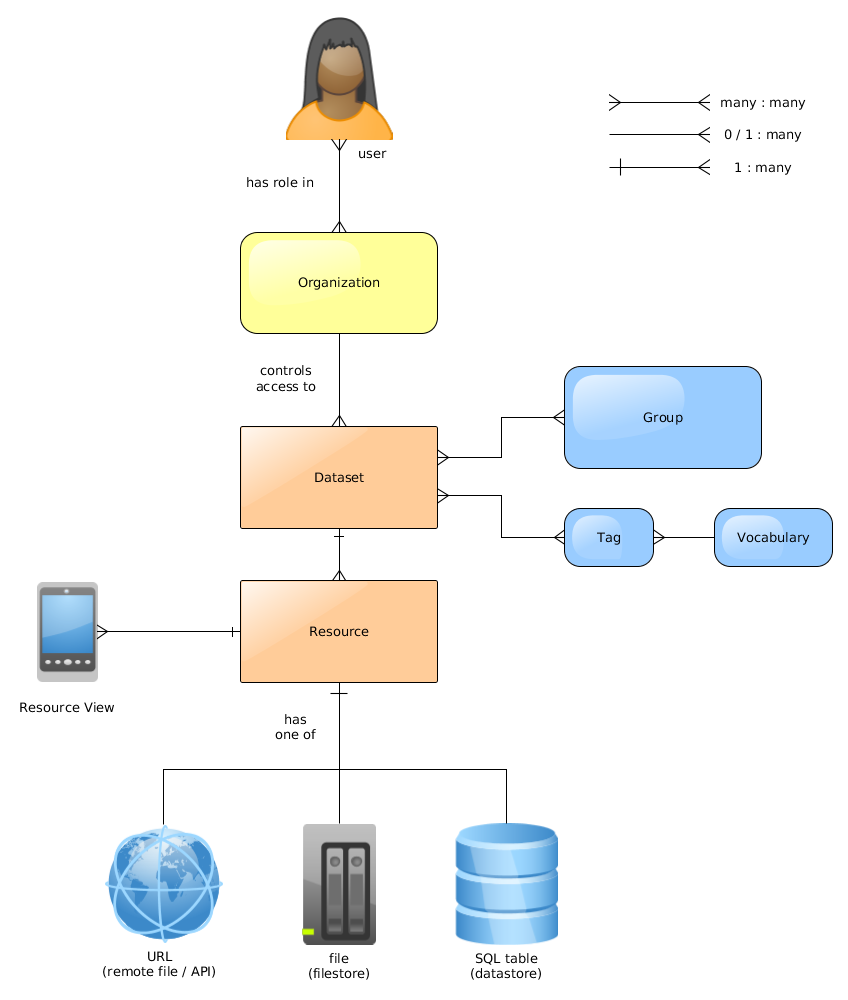
\includegraphics[width=0.7\textwidth]{ckan_model.png}
	\caption{CKAN data model}
	\label{fig:ckan_model}
\end{figure}

\subsection{DKAN}
DKAN\footnote{\url{http://nucivic.com/dkan/}} is a Drupal-based DMS with a full suite of cataloging, publishing and visualization features. Built over Drupal, DKAN can be easily customized and extended. The actual data sets in DKAN can be stored either within DKAN or on external sites. DKAN users are able to explore, search and describe datasets through the web interface or a RESTful API.

The DKAN data model\footnote{\url{http://docs.getdkan.com/dkan-documentation/dkan-developers/dataset-technical-field-reference/}} is very similar to the CKAN one, containing information to describe datasets, resources, groups and tags.

\subsection{Socrata}
Socrata\footnote{\url{http://socrata.com}} is a commercial platform to streamline data publishing, management, analysis and reusing. It empowers users to review, compare, visualize and analyze data in real time. Datasets hosted in Socrata can be accessed using RESTful API that facilitates search and data filtering.

Socrata allows flexible data management by implementing various data governance models and ensuring compliance with metadata schema standards. It also enables administrators to track data usage and consumption through dashboards with real-time reporting. Socrata is very flexible when it comes to customizations. It has a consumer-friendly experience giving users the opportunity to tell their story with data. Socrata's data model is designed to represent tabular data: it covers a basic set of metadata properties and has good support for geospatial data.

\subsection{Schema.org}
Schema.org\footnote{\url{http://schema.org}} is a collection of schemas used to markup HTML pages with structured data. This structured data allows many applications, such as search engines, to understand the information contained in Web pages, thus improving the display of search results and making it easier for people to find relevant data.

Schema.org covers many domains. We are specifically interested in the \texttt{Dataset} schema. However, there are many classes and properties that can be used to describe organizations, authors, etc.

\subsection{Project Open Data}
Project Open Data (POD)\footnote{\url{http://project-open-data.cio.gov/}} is an online collection of best practices and case studies to help data publishers. It is a collaborative project that aims to evolve as a community resource to facilitate adoption of open data practices and facilitate collaboration and partnership between both private and public data publishers.

The POD metadata model\footnote{\url{https://project-open-data.cio.gov/v1.1/schema/}} is based on DCAT. Similarly to DCAT-AP, POD defines three types of metadata elements: Required, Required-if(conditionally required) and Expanded (optional). The metadata model is presented in the JSON format and encourages publishers to extend their metadata descriptions using elements from the ``Expanded Fields'' list, or from any well-known vocabulary.

%%%%%%%%%%%%%%%%%%%%%%%%%%%%%%%%%%%%
%%%  3. Metadata Classification  %%%
%%%%%%%%%%%%%%%%%%%%%%%%%%%%%%%%%%%%

\section{Metadata Classification}
\label{section:metadata}
A dataset metadata model should contain sufficient information so that consumers can easily understand and process the data that is described. After analyzing the models described in the section~\ref{section:models}, we find out that a dataset can contain four main sections:
\begin{itemize}
  \item \textbf{Resources}: The actual raw data that can be downloaded or accessed directly via queryable endpoints. Resources can come in various formats such as JSON, XML or RDF.
  \item \textbf{Tags}: Descriptive knowledge about the dataset content and structure. This can range from simple textual representation to semantically rich controlled terms. Tags are the basis for datasets search and discovery.
  \item \textbf{Groups}: Groups act as organizational units that share common semantics. They can be seen as a cluster or a curation of datasets based on shared categories or themes.
  \item \textbf{Organizations}: Organizations are another way to arrange datasets. However, they differ from groups as they are not constructed by shared semantics or properties, but solely on the dataset's association to a specific administration party.
\end{itemize}

Upon closed examination of the various data models, we group the metadata information into eight main types. Each section discussed above should contain one or more of these types. For example, resources have general, access, ownership and provenance information while tags have general and provenance information only. The eight information types are:
\begin{itemize}
 \item \textbf{General information}: The core information about the dataset (e.g., title, description, ID). The most common vocabulary used to describe this information is Dublin Core\footnote{\url{http://dublincore.org/documents/dcmi-terms/}}.
 \item \textbf{Access information}: Information about dataset access and usage (e.g., URL, license title and license URL). In addition to the properties in the models discussed above, there are several vocabularies designed specially to describe data access right e.g. Linked Data Rights\footnote{\url{http://oeg-dev.dia.fi.upm.es/licensius/static/ldr/}}, the Open Digital Rights Language (ODRL)\footnote{\url{http://www.w3.org/ns/odrl/2/}}.
 \item \textbf{Ownership information}: Authoritative information about the dataset (e.g. author, maintainer and organization). The common vocabularies used to expose ownership information are Friend-of-Friend (FOAF)\footnote{\url{http://xmlns.com/foaf/spec/}} for people and relationships, vCard~\cite{Iannella:W3C:14} for people and organizations and the Organization ontology~\cite{Reynolds:W3C:14} designed specifically to describe organizational structures.
 \item \textbf{Provenance information}: Temporal and historical information about the dataset creation and update records, in addition to versioning information (e.g. creation data, metadata update data, latest version). Provenance information coverage varies across the modeled surveyed. However, its great importance lead to the development of various special vocabularies like the Open Provenance Model\footnote{\url{http://open-biomed.sourceforge.net/opmv/}} and PROV-O~\cite{Lebo:W3C:13}. DataID~\cite{Brummer::ICSS:14} is an effort to provide semantically rich metadata with focus on providing detailed provenance, license and access information.
 \item \textbf{Geospatial information}: Information reflecting the geographical coverage of the dataset represented with coordinates or geometry polygons. There are several additional models and extensions specifically designed to express geographical information. The Infrastructure for Spatial Information in the European Community (INSPIRE) directive\footnote{\url{http://inspire.ec.europa.eu/}} aims at establishing an infrastructure for spatial information. Mappings have been made between DCAT-AP and the INSPIRE metadata. CKAN provides as well a spatial extension\footnote{\url{https://github.com/ckan/ckanext-spatial}} to add geospatial capabilities. It allows importing geospatial metadata from other resources and supports various standards (e.g. ISO 19139) and formats (e.g. GeoJSON).
 \item \textbf{Temporal information}: Information reflecting the temporal coverage of the dataset (e.g. from date to date). There has been some notable work on extending CKAN to include temporal information. \texttt{govdata.de} is an Open Data portal in Germany that extends the CKAN data model to include information like \texttt{temporal\_granularity}, \texttt{temporal\_coverage\_to} and \texttt{temporal\_granularity\_from}.
 \item \textbf{Statistical information}: Statistical information about the data types and patterns in datasets (e.g. properties distribution, number of entities and RDF triples). This information is particularly useful to explore a dataset as it gives detailed insights about the raw data when provided properly. VoID is the only model that provides statistical information about a dataset. VoID defines properties to express different statistical characteristics of datasets like the total number of triples, total number of entities, total number of distinct classes, etc. However, there are other vocabularies such as SCOVO~\cite{Hausenblas:ESWC:09} that can model and publish statistical data about datasets.
 \item \textbf{Quality information}: Information that indicates the quality of the dataset on the metadata and instance levels. In addition to that, a dataset should include an openness score that measures its alignment with the Linked Data publishing standards~\cite{Berners-Lee:W3C:06}. Quality information is only expressed in the POD metadata. However, \texttt{govdata.de} extends the CKAN model also to include a \texttt{ratings\_average} field. Moreover, there are various other vocabularies like daQ~\cite{Debattista:WWW:14} that can be used to express datasets quality. The RDF Review Vocabulary\footnote{\url{http://vocab.org/review/}} can also be used to express reviews and ratings about the dataset or its resources.
\end{itemize}

%%%%%%%%%%%%%%%%%%%%%%%%%%%%%%%%%%%%%%%
%%%  4. Towards A Harmonised Model  %%%
%%%%%%%%%%%%%%%%%%%%%%%%%%%%%%%%%%%%%%%

\section{Towards A Harmonized Model}
\label{section:hdl}
Since establishing a common vocabulary or model is the key to communication, we identified the need for an harmonized dataset metadata model containing sufficient information so that consumers can easily understand and process datasets. To create the mappings between the different models, we performed various steps:
\begin{itemize}
  \item Examine the model or vocabulary specification and documentation.
  \item Examine existing datasets using these models and vocabularies. \url{http://dataportals.org} provides a comprehensive list of Open Data Portals from around the world. It was our entry point to find out portals using CKAN or DKAN as their underlying DMS. We also investigated portals known to be using specific DMS. Socrata, for example, maintains a list of Open Data portals using their software on their homepage such as \url{http://pencolorado.org} and \url{http://data.maryland.gov}.
  \item Examine the source code of some portals. This was specifically the case for Socrata as their API returns the raw data serialized as JSON rather than the dataset's metadata. As a consequence, we had to investigate the Socrata Open Data API (SODA) source code\footnote{https://github.com/socrata/soda-java/tree/master/src/main/java/com/socrata/model} and check the different classes and interfaces.
\end{itemize}

\begin{table}[!htbp]
\centering
\tiny
\begin{tabular}{|l|l|l|l|l|l|l|}
\hline
\multicolumn{1}{|c|}{\textbf{CKAN}} & \multicolumn{1}{c|}{\textbf{DKAN}} & \multicolumn{1}{c|}{\textbf{POD}} & \multicolumn{1}{c|}{\textbf{DCAT}}     & \multicolumn{1}{c|}{\textbf{VoID}}     & \multicolumn{1}{c|}{\textbf{Schema.org}} & \multicolumn{1}{c|}{\textbf{Socrata}} \\ \hline
resources                           & resources                          & distribution                      & dcat:Distribution                      & void:Dataset$\rightarrow$ void:dataDump & Dataset:distribution                    & attachments                           \\ \hline
tags                                & tags                               & keyword                           & dcat:Dataset$\rightarrow$ :keyword   & void:Dataset$\rightarrow$ :keyword   & CreativeWork:keywords                     & tags                                  \\ \hline
groups                              & groups                             & theme                             & dcat:Dataset$\rightarrow$ :theme     &   \multicolumn{1}{c|}{-}                                      & CreativeWork:about                       & category                              \\ \hline
organization                        & organization                       & publisher                         & dcat:Dataset$\rightarrow$ :publisher &   void:Dataset$\rightarrow$ :publisher                                     & \multicolumn{1}{c|}{-}                   & \multicolumn{1}{c|}{-}                                      \\ \hline
\end{tabular}
\caption{Data models sections mapping}
\label{tab:models_section_mappings}
\end{table}

The first task is to map the four main information sections (resources, tags, groups and organization) across those models. Table~\ref{tab:models_section_mappings} shows our proposed mappings. For the ontologies (DCAT, VoID), the first part represents the class and the part after $\rightarrow$ represents the property. For Schema.org, the first part refers to the schema and the second part after $:$ refers to the property.

Table~\ref{tab:harmonized_dataset_models_mappings} presents the full mappings between the models across the information groups. Entries in the CKAN marked with $\ast$ are properties from CKAN extensions and not included in the original data model. Similar to the sections mappings, for the ontologies (DCAT, VoID), the first part represents the class and the part after $\rightarrow$ represents the property. However, sometimes the part after $\rightarrow$ refers to another resource. For example, to describe the dataset's maintainer email in DCAT, the information should be presented in the \texttt{dcat:Dataset} class using the \texttt{dcat:contactPoint} property. However, the range of this property is a resource of type \texttt{vcard} which has the property \texttt{hasEmail}.

For Schema.org, similar to the sections mapping, the first part refers to the schema and the second part after $:$ refers to the property. However, if the property is inherited from another schema we denote that by using a $\rightarrow$ as well. For example, the size of a dataset is a property for a \texttt{Dataset} schema specified in its \texttt{distribution} property. However, the type of \texttt{distribution} is \texttt{dataDownload} which is inherited from the \texttt{MediaObject} schema. The size for \texttt{MediaObject} is defined in its \texttt{contentSize} property which makes the mapping string \texttt{Dataset:distribution$\rightarrow$ DataDownload$\rightarrow$ MediaObject:contentSize}.

Examining the different models, we noticed a lack of a complete model that covers all the information types. There is an abundance of extensions and application profiles that try to fill in those gaps, but they are usually domain specific addressing specific issues like geographic or temporal information. To the best of our knowledge, there is still no complete model that encompasses all the described information types.

HDL aims at filling this gap by taking the best from these models. HDL is currently modeled in JSON\footnote{\url{https://github.com/ahmadassaf/opendata-checker/blob/master/model/hdl.json}} but converting it to a standalone OWL ontology is part of our future work.

The CKAN model controls the values to be used in describing some dataset properties. For example, the \texttt{resource\_type} property can have the values: file: direct accessible bitstream, file.upload: file uploaded to the CKAN FileStore\footnote{\url{http://docs.ckan.org/en/ckan-1.8/filestore.html}}, api, visualization, code: the actual source code or a reference to a code repository and documentation. However, using the Roomba tool~\cite{Assaf:WWW:15}, we managed to generate portal-wide reports about the representation of various fields in CKAN portals. The goal behind these reports is to find what are the frequent fields data publishers are adding as \texttt{extras} fields.

We created two ``key:object meta-field values'' reports using Roomba. The first one aims to collect the list of \texttt{extras} values using the query string\\ \texttt{extras>value:extras>name} and the second one is to list the file types specified for resources using the query string \texttt{resources>resource\_type:resources>name}. We run the report generation process on two prominent data portals: the Linked Open Data (LOD) cloud hosted on the Datahub containing 259 datasets and the Africa's largest open data portal, OpenAfrica\footnote{\url{http://africaopendata.org/}} that contains 1653 datasets.

After examining the results, we noticed that for OpenAfrica, 53\% of the datasets contained additional information about the geographical coverage of the dataset (e.g. spatial-reference-system, spatial\_harvester, bbox-east-long, bbox-north-long, bbox-south-long, bbox-west-long). In addition, 16\% of the datasets have additional provenance and ownership information (e.g frequency-of-update, dataset-reference-date). For the LOD cloud, the main information embedded in the extras fields are about the structure and statistical distribution of the dataset (e.g. namespace, number of triples and links). The OpenAfrica resources did not specify any extra resource types. However, in the LOD cloud, we observe that multiple resources define additional types (e.g. example, api/sparql, publication, example).

Roomba easily enables to perform such tests and to gather a detailed view about the kind of missing information data publishers require in the core model. We further plan to run Roomba on various portals to collect more information about such missing data to include it in HDL.

\newgeometry{outer=20mm,inner=20mm,vmargin=10mm,includehead,includefoot,headheight=20pt}
\pagestyle{lscape}
\begin{landscape}
\Huge
\noindent
\setlength\LTleft{-1.7cm}
{\tiny
\begin{longtable}{|p{1cm}|m{3.1cm}|m{2.4cm}|m{2.5cm}|p{3.8cm}|m{3.8cm}|m{5.55cm}|m{2.5cm}|}
\caption[Harmonized Dataset Models Mappings]{Harmonized Dataset Models Mappings} \label{tab:harmonized_dataset_models_mappings} \\

\hline \multicolumn{1}{|p{2cm}}{\textbf{Data Model}} & \multicolumn{1}{|c|}{\textbf{CKAN}} & \multicolumn{1}{c|}{\textbf{DKAN}} & \multicolumn{1}{c|}{\textbf{POD}} & \multicolumn{1}{c|}{\textbf{DCAT}} & \multicolumn{1}{c|}{\textbf{VoID}} & \multicolumn{1}{c|}{\textbf{Schema.org}} & \multicolumn{1}{c|}{\textbf{Socrata}}\\ \hline
\endfirsthead

\multicolumn{8}{c}
{{\bfseries \tablename\ \thetable{} Harmonized Dataset Models Mappings}} \\
\hline \multicolumn{1}{|p{2cm}}{\textbf{Data Model}} &
\multicolumn{1}{c|}{\textbf{CKAN}} &
\multicolumn{1}{c|}{\textbf{DKAN}} &
\multicolumn{1}{c|}{\textbf{POD}} &
\multicolumn{1}{c|}{\textbf{DCAT}} &
\multicolumn{1}{c|}{\textbf{VoID}} &
\multicolumn{1}{c|}{\textbf{Schema.org}} &
\multicolumn{1}{c|}{\textbf{Socrata}} \\ \hline
\endhead

\hline
\endfoot

\endlastfoot

\multirow{13}{2cm}{General Information} & id & id & identifier & dcat:Dataset$\rightarrow$ dct:identifier &  &  & id/externalId\tabularnewline
\cline{2-8}
 & private & private & accessLevel &  &  &  & privateMetadata\tabularnewline
\cline{2-8}
 & state & state &  &  &  &  & publicationStage\tabularnewline
\cline{2-8}
 & type & type &  &  &  & Thing:additionalType & \tabularnewline
\cline{2-8}
 & name & name &  &  &  & Thing:name & name\tabularnewline
\cline{2-8}
 & isopen &  &  &  &  &  & \tabularnewline
\cline{2-8}
 & notes & notes & description & dcat:Dataset$\rightarrow$ dct:description & void:Dataset$\rightarrow$ dct:description & Thing:description & description\tabularnewline
\cline{2-8}
 & title & title & title & dcat:Dataset$\rightarrow$ dct:title & void:Dataset$\rightarrow$ dc:title & Thing:name & name\tabularnewline
\cline{2-8}
 & num\_resources &  &  &  & void:Dataset$\rightarrow$ void:documents &  & \tabularnewline
\cline{2-8}
 & num\_tags &  &  &  &  &  & \tabularnewline
\cline{2-8}
 &  &  & conformsTo & dcat:Dataset$\rightarrow$ dct:conformsTo & void:Dataset$\rightarrow$ dct:conformsTo &  & \tabularnewline
\cline{2-8}
 &  &  & language & dcat:Dataset$\rightarrow$ dct:language & void:Dataset$\rightarrow$ dct:language & CreativeWork:inLanguage & \tabularnewline
\cline{2-8}
 &  &  & accuralPeriodicity & dcat:Dataset$\rightarrow$ dct:accuralPeriodicity & void:Dataset$\rightarrow$ dct:accuralPeriodicity &  & \tabularnewline
\hline
\multirow{7}{2cm}{access information} & license\_title & license\_title & license & dcat:Distribution$\rightarrow$ dct:license & void:Dataset$\rightarrow$ dct:license &  & license$\rightarrow$  name\tabularnewline
\cline{2-8}
 & license\_id &  &  &  &  &  & licenseId\tabularnewline
\cline{2-8}
 & license\_url &  &  &  &  & CreativeWork:license & license $\rightarrow$  termsLink\tabularnewline
\cline{2-8}
 & url & url & landingPage & dcat:Dataset$\rightarrow$ dcat:landingPage &  & Thing:url & \tabularnewline
\cline{2-8}
 &  &  & rights & dcat:Distribution$\rightarrow$  dct:rights & void:Dataset$\rightarrow$ dct:rights &  & \tabularnewline
\cline{2-8}
 & attribution\_text$\ast$ &  &  &  &  &  & attribution\tabularnewline
\cline{2-8}
 &  &  &  &  &  &  & attributionLink\tabularnewline
\hline
\multirow{7}{2cm}{provenance} & version &  &  &  &  & CreativeWork:version & \tabularnewline
\cline{2-8}
 & revision\_id &  &  &  &  &  & \tabularnewline
\cline{2-8}
 & metadata\_created & metadata\_created &  & dcat:Distribution$\rightarrow$ dct:created & void:Dataset$\rightarrow$ dct:created & CreativeWork:dateCreated & \tabularnewline
\cline{2-8}
 & metadata\_modified & metadata\_modified & modified & dcat:Distribution$\rightarrow$ dct:modified & void:Dataset$\rightarrow$ dct:modified & CreativeWork:dateModified & \tabularnewline
\cline{2-8}
 & revision\_timestamp & revision\_timestamp &  &  &  &  & \tabularnewline
\cline{2-8}
 &  &  & issued & dcat:Distribution$\rightarrow$ dct:issued & void:Dataset$\rightarrow$ dct:issued & CreativeWork:datePublished & \tabularnewline
\cline{2-8}
 &  &  & temporal & dcat:Dataset$\rightarrow$ dct:temporal & void:Dataset$\rightarrow$ dct:temporal & Dataset:temporal & \tabularnewline
\hline
\multirow{14}{2cm}{ownership} & maintainer & maintainer & contactPoint$\rightarrow$ fn & dcat:Dataset$\rightarrow$ dcat:contactPoint$\rightarrow$ vcard:fn &  & CreativeWork:producer$\rightarrow$ Thing:name & owner$\rightarrow$ displayName / owner$\rightarrow$ ScreenName\tabularnewline
\cline{2-8}
 & maintainer\_email & maintainer\_email & contactPoint$\rightarrow$ hasEmail & dcat:Dataset$\rightarrow$ dcat:contactPoint$\rightarrow$ vcard:hasEmail &  & CreativeWork:producer$\rightarrow$ Person:email & \tabularnewline
\cline{2-8}
 & owner\_org &  &  &  &  & CreativeWork:sourceOrganization:LegalName & \tabularnewline
\cline{2-8}
 & author &  &  & dcat:Dataset$\rightarrow$ dct:creator$\rightarrow$ foaf:Person:givenName & void:Dataset$\rightarrow$ dct:creator$\rightarrow$ foaf:Person:givenName & CreativeWork:author$\rightarrow$ Thing:name & \tabularnewline
\cline{2-8}
 & author\_email & author\_email &  & dcat:Dataset$\rightarrow$ dct:creator$\rightarrow$ foaf:Person:mbox & void:Dataset$\rightarrow$ dct:creator$\rightarrow$ foaf:Person:mbox & CreativeWork:author$\rightarrow$ Person:email & \tabularnewline
\cline{2-8}
 &  &  & bureauCode &  &  &  & \tabularnewline
\cline{2-8}
 &  &  & programCode &  &  &  & \tabularnewline
\cline{2-8}
 & description &  &  &  &  & CreativeWork:sourceOrganization$\rightarrow$ Thing:description & \tabularnewline
\cline{2-8}
 &  &  & isPartOf &  &  & CreativeWork:isPartOf & \tabularnewline
\cline{2-8}
 &  &  &  &  &  & CreativeWork:hasPart & \tabularnewline
\cline{2-8}
 &  &  & systemOfRecords &  &  &  & \tabularnewline
\cline{2-8}
 &  &  & describedBy &  &  &  & \tabularnewline
\cline{2-8}
 &  &  & describedByType &  &  &  & \tabularnewline
\hline
\multirow{6}{2cm}{GeoSpatial} & spatial-text$\ast$ &  & spatial & dcat:Dataset$\rightarrow$ dct:spatial & void:Dataset$\rightarrow$ dct:spatial & Dataset:spatial & \tabularnewline
\cline{2-8}
 & geographical\_granularity$\ast$ &  &  &  &  &  & \tabularnewline
\cline{2-8}
 &  &  &  &  &  &  & bbox\tabularnewline
\cline{2-8}
 &  &  &  &  &  &  & layers\tabularnewline
\cline{2-8}
 &  &  &  &  &  &  & bboxCrs\tabularnewline
\cline{2-8}
 &  &  &  &  &  &  & namespace\tabularnewline
\hline
\multirow{4}{2cm}{Temporal} &  &  & temporal & dcat:Dataset$\rightarrow$ dct:temporal & void:Dataset$\rightarrow$ dct:temporal & Dataset:temporal & \tabularnewline
\cline{2-8}
 & temporal\_granularity$\ast$ &  &  &  &  &  & \tabularnewline
\cline{2-8}
 & temporal\_coverage\_to$\ast$ &  &  &  &  &  & \tabularnewline
\cline{2-8}
 & temporal\_coverage\_from$\ast$ &  &  &  &  &  & \tabularnewline
\hline
Quality & ratings\_average$\ast$ &  & dataQuality &  &  & CreativeWork:aggregateRating & \tabularnewline
\hline
\multicolumn{8}{|c|}{\cellcolor{blue!25}\textbf{Organization}}\tabularnewline
\hline
\multirow{10}{2cm}{General Information} & title &  & name & dcat:Dataset$\rightarrow$ dct:creator$\rightarrow$ foaf:Organization:givenName & void:Dataset$\rightarrow$ dct:creator$\rightarrow$ foaf:Organization:givenName & CreativeWork:sourceOrganization:LegalName & \tabularnewline
\cline{2-8}
 & description &  &  &  &  & CreativeWork:sourceOrganization$\rightarrow$ Thing:description & \tabularnewline
\cline{2-8}
 & id &  &  &  &  &  & \tabularnewline
\cline{2-8}
 & type &  &  &  &  & CreativeWork:sourceOrganization$\rightarrow$ Thing:additionalType & \tabularnewline
\cline{2-8}
 & name &  &  &  &  & CreativeWork:sourceOrganization$\rightarrow$ Thing:name & \tabularnewline
\cline{2-8}
 & image\_url &  &  &  &  &  & \tabularnewline
\cline{2-8}
 & state &  &  &  &  &  & \tabularnewline
\cline{2-8}
 & is\_organization &  &  &  &  &  & \tabularnewline
\cline{2-8}
 & approval\_status &  &  &  &  &  & \tabularnewline
\cline{2-8}
 &  &  & subOrganizationOf &  &  & CreativeWork:sourceOrganization:subOrganization & \tabularnewline
\multirow{2}{2cm}{provenance} & revision\_timestamp &  &  &  &  &  & \tabularnewline
\cline{2-8}
 & revision\_id &  &  &  &  &  & \tabularnewline
\hline
\multicolumn{8}{|c|}{\cellcolor{blue!25}\textbf{Resources}}\tabularnewline
\hline
\multirow{15}{2cm}{general} & resource\_group\_id & resource\_group\_id &  &  &  &  & \tabularnewline
\cline{2-8}
 & id & id &  &  &  &  & blobId\tabularnewline
\cline{2-8}
 & size & size &  & dcat:Distribution$\rightarrow$ dcat:byteSize &  & Dataset:distribution$\rightarrow$ DataDownload$\rightarrow$ MediaObject:contentSize & \tabularnewline
\cline{2-8}
 & state & state &  &  &  &  & \tabularnewline
\cline{2-8}
 & hash &  &  &  &  &  & \tabularnewline
\cline{2-8}
 & description & description & description & dcat:Distribution$\rightarrow$ dct:description &  & Dataset:distribution$\rightarrow$ DataDownload$\rightarrow$ Thing:description & \tabularnewline
\cline{2-8}
 & format & format & format & dcat:Distribution$\rightarrow$ dct:format & void:Dataset$\rightarrow$ dct:format & Dataset:distribution$\rightarrow$ DataDownload$\rightarrow$ MediaObject:encodingFormat & \tabularnewline
\cline{2-8}
 & mimetype & mimetype & mediaType & dcat:Distribution$\rightarrow$ dcat:mediaType &  &  & \tabularnewline
\cline{2-8}
 & mimetype\_inner &  &  &  &  &  & \tabularnewline
\cline{2-8}
 & name & name & title & dcat:Distribution$\rightarrow$ dct:title &  & Dataset:distribution$\rightarrow$ DataDownload$\rightarrow$ Thing:name & filename / name\tabularnewline
\cline{2-8}
 & position &  &  &  &  &  & \tabularnewline
\cline{2-8}
 & resource\_type &  &  &  &  & Dataset:distribution$\rightarrow$ DataDownload$\rightarrow$Thing:additionalType & \tabularnewline
\cline{2-8}
 &  &  & describedBy &  &  &  & \tabularnewline
\cline{2-8}
 &  &  & describedByType &  &  &  & \tabularnewline
\cline{2-8}
 &  &  & conformsTo &  &  &  & \tabularnewline
\hline
\multirow{5}{2cm}{access information} & cache\_url &  &  &  &  &  & \tabularnewline
\cline{2-8}
 & url-type &  &  &  &  &  & \tabularnewline
\cline{2-8}
 & url & url & downloadURL & dcat:Distribution$\rightarrow$ dcat:downloadURL & void:Dataset$\rightarrow$ void:dataDump & Dataset:distribution$\rightarrow$ DataDownload$\rightarrow$ Thing:url & \tabularnewline
\cline{2-8}
 &  &  & accessURL & dcat:Distribution$\rightarrow$ dcat:accessURL &  & Dataset:distribution$\rightarrow$ DataDownload$\rightarrow$ MediaObject:contentUrl & accessPoints\tabularnewline
\cline{2-8}
 & webstore\_url &  &  &  &  &  & \tabularnewline
\hline
\multirow{6}{2cm}{provenance} & cache\_last\_updated &  &  &  &  &  & \tabularnewline
\cline{2-8}
 & revision\_timestamp & revision\_timestamp &  &  &  &  & \tabularnewline
\cline{2-8}
 & webstore\_last\_updated &  &  &  &  &  & \tabularnewline
\cline{2-8}
 & created & created &  &  &  & Dataset:distribution$\rightarrow$ DataDownload$\rightarrow$ CreativeWork:dataCreated & created\_at\tabularnewline
\cline{2-8}
 & last\_modified & last\_modified &  &  &  & Dataset:distribution$\rightarrow$ DataDownload$\rightarrow$ CreativeWork:dataModified & updated\_at\tabularnewline
\cline{2-8}
 & revision\_id & revision\_id &  &  &  &  & \tabularnewline
\hline
\multicolumn{8}{|c|}{\cellcolor{blue!25}\textbf{Groups}}\tabularnewline
\hline
\multirow{7}{2cm}{General} & display\_name & display\_name &  &  &  &  & \tabularnewline
\cline{2-8}
 & description & description &  &  &  &  & \tabularnewline
\cline{2-8}
 & title & title &  &  &  &  & \tabularnewline
\cline{2-8}
 & image\_display\_url & image\_display\_url &  &  &  &  & \tabularnewline
\cline{2-8}
 & id & id &  &  &  &  & \tabularnewline
\cline{2-8}
 & name & name &  &  &  &  & \tabularnewline
\cline{2-8}
 & subgroups$\ast$ &  &  &  &  &  & \tabularnewline
\hline
\multicolumn{8}{|c|}{\cellcolor{blue!25}\textbf{Tags}}\tabularnewline
\hline
\multirow{5}{2cm}{General} & vocabulary\_id & vocabulary\_id &  & dcat:Dataset$\rightarrow$ dcat:theme$\rightarrow$ skos:ConceptScheme &  &  & \tabularnewline
\cline{2-8}
 & display\_name &  &  & dcat:Dataset$\rightarrow$ dcat:keyword &  &  & \tabularnewline
\cline{2-8}
 & name & name &  & dcat:Dataset$\rightarrow$ dcat:theme$\rightarrow$ skos:Concept &  &  & \tabularnewline
\cline{2-8}
 & state &  &  &  &  &  & \tabularnewline
\cline{2-8}
 & id & id &  &  &  &  & \tabularnewline
\hline
Provenance & revision\_timestamp &  &  &  &  &  & \tabularnewline
\hline
\end{longtable}
}
\end{landscape}

\restoregeometry
\pagestyle{standard}